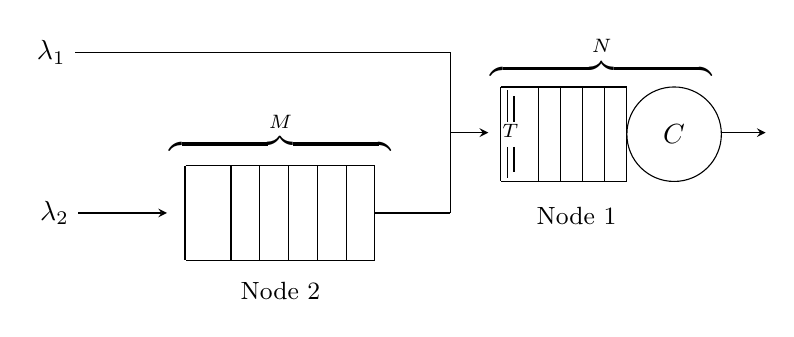
\begin{tikzpicture}[>=stealth, scale=0.8],
    % the rectangle of Queue 1
    \draw (0,0) -- ++(3cm,0) -- ++(0,-1.5cm) -- ++(-3cm,0);
    % The label above Queue 1 -> M
    \node[anchor=north] at (1.5cm, 1cm) {\(
        \overbrace{\qquad \qquad \qquad \qquad}^{M}
    \)};
    % The label below Queue 1 -> Node 2
    \node[anchor=north] at (1.5cm, -1.7cm) {\small{Node 2}};

    % the vertical lines in Queue 1
    \foreach \i in {1,...,5, 6.6}
    \draw (3cm-\i*13pt,0) -- +(0,-1.5cm);

    % % the circle in Queue 1
    % \draw (2.75,-0.75cm) circle [radius=0.75cm] node {\(0\)};

    % the rectangle in Queue 2
    \draw (5,1.25) -- ++(2cm,0) -- ++(0,-1.5cm) -- ++(-2cm,0);
    % the vertical lines in Queue 2
    \foreach \i in {1,...,4, 5.7}
    \draw (7cm-\i*10pt,1.25) -- +(0,-1.5cm);
    % The two vertical lines at the start of Queue 2
    \draw (7cm-54pt,1.2) -- +(0,-0.5cm);
    \draw (7cm-54pt,0.3) -- +(0,-0.5cm);
    \draw (7cm-51pt,1.1) -- +(0,-0.4cm);
    \draw (7cm-51pt,0.3) -- +(0,-0.4cm);

    % The label between the lines for T
    \node[anchor=north] at (5.15, 0.81 cm) {\scriptsize \( T \)};

    % The label above Queue 2 -> N
    \node[anchor=north] at (6.6cm, 2.2cm) {\(
        \overbrace{\qquad \qquad \qquad \qquad}^{N}
    \)};
    % The label below Queue 2 -> Node 1
    \node[anchor=north] at (6.2cm, -0.5cm) {\small{Node 1}};

    % the circle in Queue 2
    \draw (7.75,0.5) circle [radius=0.75cm] node {\(C\)};

    % Arrow line from Queue 2 outside
    \draw[->] (8.5,0.525) -- +(20pt,0);

    % Line from lambda_2 to Queue 1
    \draw[<-] (-0.3,-0.75) -- +(-40pt,0) node[left] {\( \lambda_2 \)};
    % First line (horizontal) after Queue 1
    \draw[-] (3,-0.75) -- +(34pt,0);
    % Second line (vertical) after Queue 1
    \draw (4.2, 0.525) -- (4.2, -0.75);

    % First line (horizontal) from lambda_1
    \draw (4.2, 1.8) -- +(-169.5pt,0) node[left] {\( \lambda_1 \)};
    % Second line (vertical) from lambda_1
    \draw (4.2, 1.8) -- (4.2, 0.525);
    % Arrow line to Queue 2
    \draw[->] (4.2, 0.525) -- (4.8, 0.525);
\end{tikzpicture}
